\section{Technical Architecture}

The \gls{qnx} avionics stack will be composed of multiple modules:

\begin{enumerate}
    \setlength{\itemsep}{1pt}
    \setlength{\parskip}{0pt} \setlength{\parsep}{0pt}
    \item controller
    \item fetcher
    \item packager
    \item broadcaster
    \item writer
\end{enumerate}

\subsection{Architecture Diagrams}

The architecture for the \glsxtrshort{cuinspace} telemetry system is separated into two system designs:
\begin{enumerate}
    \setlength{\itemsep}{1pt}
    \setlength{\parskip}{0pt} \setlength{\parsep}{0pt}
    \item Critical functionality for the 2023-2024 telemetry system (Figure \ref{fig:crit-arc})
    \item Non-critical functionality which can be postponed to 2024-2025 (Figure \ref{fig:non-crit-arc})
\end{enumerate}

\begin{figure}[H]
    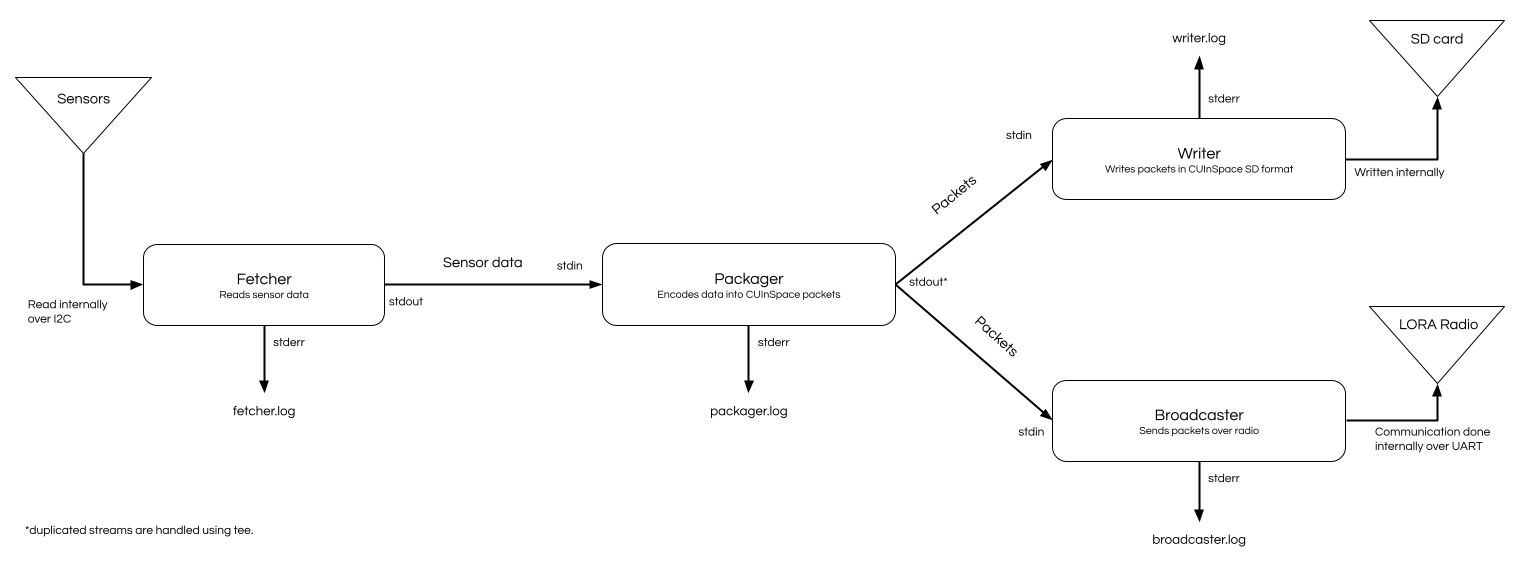
\includegraphics[width=\linewidth]{assets/critical-architecture.png}
    \caption{System diagram of the critical functionality for the telemetry system}
    \label{fig:crit-arc}
\end{figure}

\begin{figure}[H]
    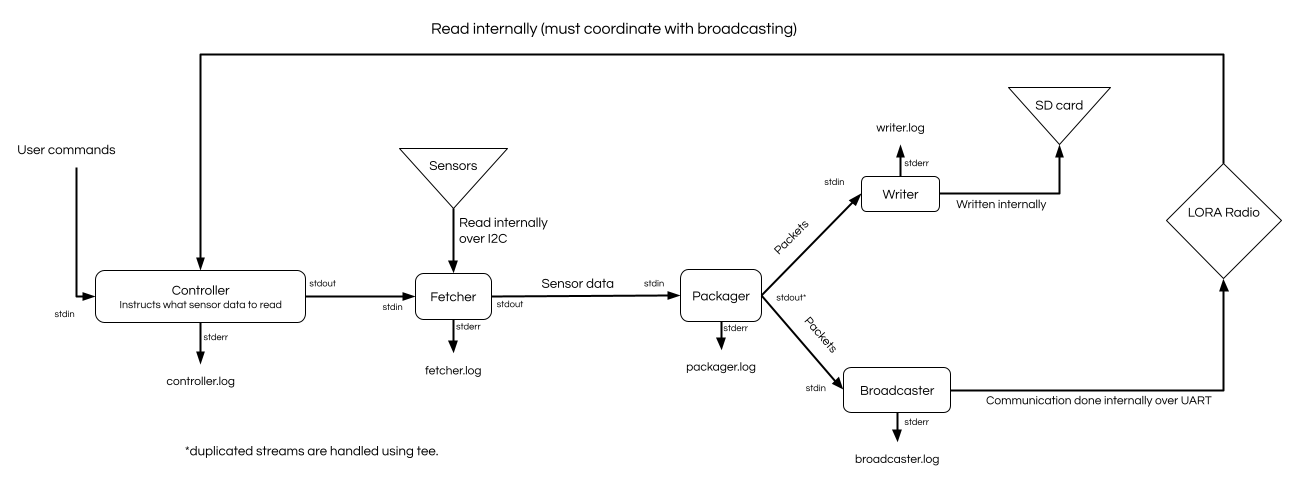
\includegraphics[width=\linewidth]{assets/non-critical-architecture.png}
    \caption{System diagram of the non-critical functionality for the telemetry system}
    \label{fig:non-crit-arc}
\end{figure}

\subsection{Modules}

Each module makes use of the \gls{unix} philosophy: do one task, and do it well. They are all \glsxtrfull{posix}
compliant in order to be portable across other \glsxtrshort{posix} compliant \glsxtrshort{rtos}s. As part of this
philosophy, each module will also take their input as plain-text (where applicable) and provide their output in plain
text as well. This allows each module's output to be useful on its own as well as part of the whole system, rather than
being tailored for input into another module. Additionally, a plain-text output makes it easier for developers to
reason about and debug module output.

All of the modules are written in the C programming language, in order to make use of \glsxtrshort{qnx}'s included C
libraries. This also facilitates \glsxtrshort{srad} development, as members in the engineering and computer science
programs become familiar with C programming early in their undergraduate degree.

All modules use \gls{stdin}, \gls{stdout} and \gls{stderr} for \glsxtrfull{ipc}. Error messages and logs are sent to
\gls{stderr} so that they can be easily separated from other program output and redirected to a log file. Modules read
their input from \gls{stdin} to be processed, and write their output to \gls{stdout}. This allows for modules to be
piped into each other easily. Modules will also be able to read from a file or a \gls{fifo} in addition to \gls{stdin}
for more control using output duplication with the \gls{posixgls} 'tee' command.

None of the libraries created for use in the modules make assumptions about memory allocation, and instead accept
pre-allocated memory blocks to initialize with data. This allows modules to be portable to embedded systems with less
overhead.

All modules are bundled with help text which can be displayed with the 'use' command. The help text contains a
description of the module, its usage, example calls, and command line options and their default values.

All modules follow the gnu11 C standard. This standard was selected because it is a modern C standard which permits the
use of \gls{gnu} libraries (such as \textit{getopt}, a library for POSIX compliant command line interfaces).

\subsubsection{Controller}

This module is not part of the critical functionality for the 2023-2024 \glsxtrshort{cuinspace} telemetry system.

The \textit{controller} module is responsible for receiving control commands from the ground station over
\glsxtrshort{lora} and providing them to \textit{fetcher} for interpretation.

The \glsxtrshort{cuinspace} packet format specification describes control packets which allow the ground station to
request only specific types of telemetry data from the rocket telemetry system. The \textit{controller} module will
read these control packets from the \glsxtrshort{lora} RN2483 chip and provide them as plain-text instructions to the
\textit{fetcher} module.

The \textit{controller} module will also be able to provide signal reports and check the \glsxtrshort{lora} radio
settings. It may later be required to take input from an interactive terminal interface so that the telemetry system
can be monitored by developers. The module will also have the ability to modify radio parameters in accordance with the
control packets it receives from the ground station.

\subsubsection{Fetcher}

The \textit{fetcher} module is responsible for constantly reading sensor data. It does so by reading data from all the
sensors on the \glsxtrshort{cuinspace} \glsxtrshort{srad} sensor board via an \glsxtrshort{i2c} bus.

The \textit{fetcher} module will output sensor data in plain-text, human readable measurements via \gls{stdout}.
Outputted sensor data will be annotated with its data type (altitude, temperature, etc.) and unit of measurement.

The \textit{fetcher} module will be able to receive instructions about which sensor data to prioritize via \gls{stdin}.
It will also be able to accept a configuration which specifies sensor addresses, sensor data types (altitude,
temperature, etc.) and commands for reading from the sensors in order to be configurable for different
\glsxtrshort{srad} sensor boards. This functionality is not part of the critical requirements for the 2023-2024
telemetry system.

\subsubsection{Packager}

The \textit{packager} module is responsible for packaging sensor data output by \textit{fetcher} into the
\glsxtrshort{cuinspace} telemetry packet format. It requires an HAM radio call sign provided via command line in order
to sign all the packets that it creates. \textit{packager} will write the encoded radio packets to \gls{stdout} in
plain-text hexadecimal digits.

\subsubsection{Broadcaster}

The \textit{broadcaster} module is responsible for interfacing with the \glsxtrshort{lora} RN2483 radio chip over UART
to broadcast messages to the ground station. It accepts input in the form of plain-text hexadecimal digits over
\gls{stdin} (or a file), which it sends to the radio chip for transmission. Newline characters in the input signify the
end of a transmission.

\textit{broadcaster} will accept command line options for all of the configurable radio parameters provided by the
RN2483 radio chip, which it will use for transmission.

\subsubsection{Writer}

The \textit{writer} module is responsible for writing \glsxtrshort{cuinspace} telemetry packets to an SD card using the
\glsxtrshort{cuinspace} SD card storage format.
